\chapter{Similar applications}

Neural Network Models as well as Machine Learning algorithms provide various versatile and adaptive methods for non-linear problem solving. Because of these reasons, there are numerous applications which perform the task of musical/audio classification using the aforementioned techniques. We will discuss in the following sections about three of those applications.

\section{Spektrum}

Spektrum is a multi-platform music genre classificator and music recommandation system developed in the context of the course "Application Challenges for
Machine Learning on the example of IBM Power AI", by the team consisting of Marte Vinje, Moritz Klimmek, Thomas Salzer, Aaron Hümmecke, Lukas Vorwerk \cite{spektrum} . The application consists of two parts:
\begin{itemize}
	\item Music Genre Classification: Performed by a Convolutional Neural Network Model which analyzes the MEL spectrogram of a given input song.
	\item Music Recommendation: Generating suggestions by making use of a combination collaborative filtering
		and content based filtering.
\end{itemize}

\begin{center}
	\centering
	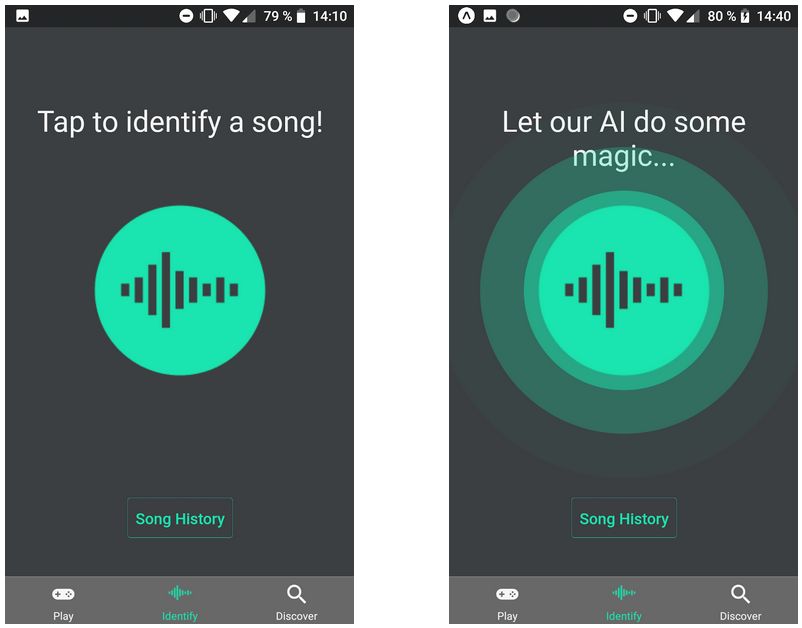
\includegraphics[width = 5.0in]{images/spektrum.png}
	\centerline{\captionof{Figure 1.1: The interface of the Spektrum application (Photo source: \cite{spektrum})}}
\label{spektrum}
\end{center}


\section{MuseNet}

MuseNet is a Deep Neural Network Framework developed by OpenAI that can generate 4-minute snippets of original musical composition
with up to 10 different instruments, combining various styles ranging from Mozart to The Beatles.
MuseNet creates music by determining the patterns over a given style as input, generating  the respective sequence of notes and chords. It also computes a relational graph between its various current styles, in order to incorporate as many related musical features as possible.

\begin{center}
	\centering
	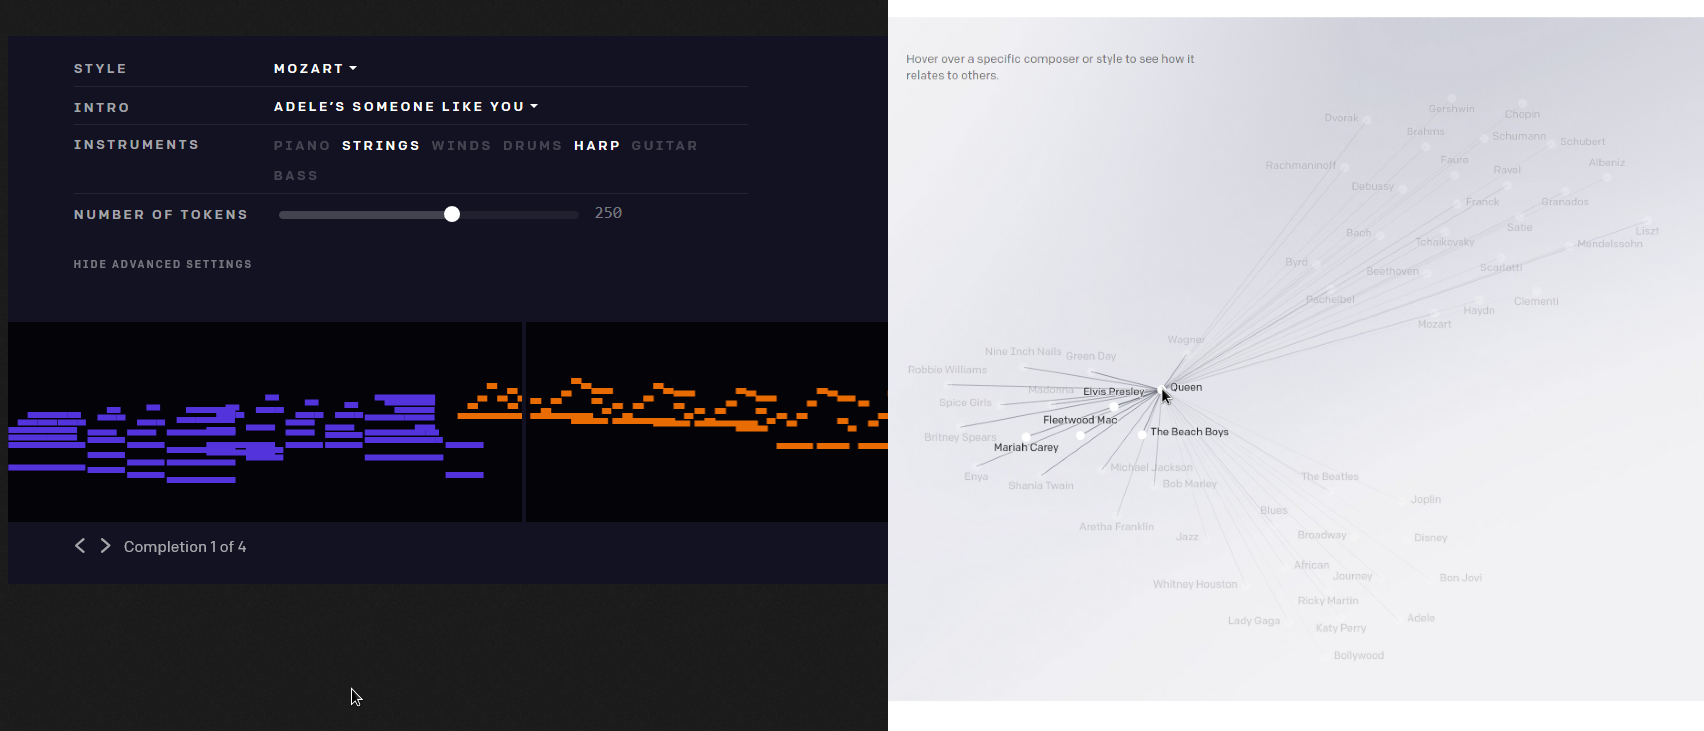
\includegraphics[width = 5.0in]{images/musenet.png}
	\centerline{\captionof{Figure 1.2: An illustration of the MuseNet's functionalities (Photo sources : \cite{musenet})}}
\label{musenet}
\end{center}

\section{Magenta}

Magenta is an open source project (started by a group of engineers from the Google Brain team), based on deep learning and reinforcement learning used for generating
and creating art. By using the Google Tensorflow as well as Magenta.js, the application produces original songs, images, drawings and material textures.

\begin{center}
	\centering
	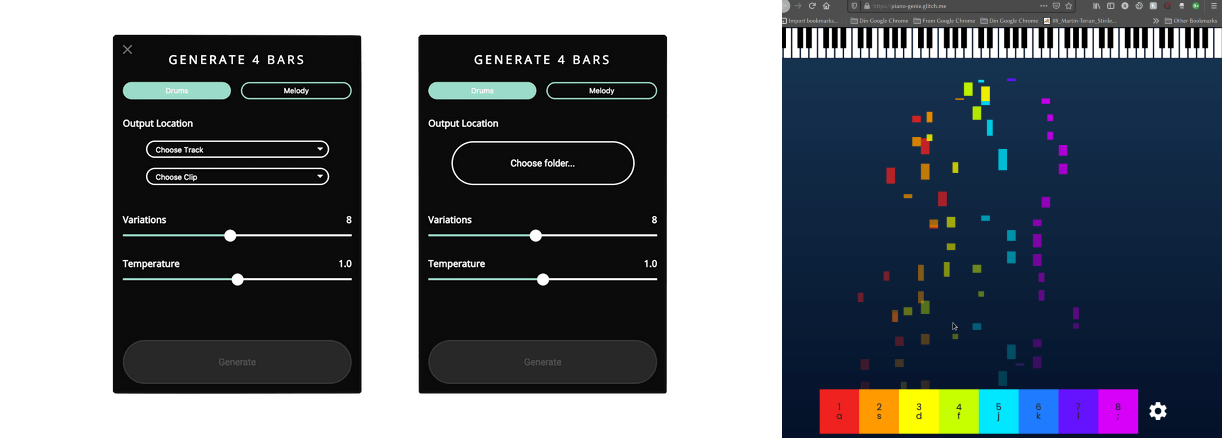
\includegraphics[width = 5.5in]{images/magenta.png}
	\centerline{\caption{Figure 1.3: Applications based on Magenta (Photo sources: \cite{magenta})}}
\label{magenta}
\end{center}
